\documentclass[../main.tex]{subfiles}
% !TeX root = ../main.tex
\begin{document}
	\section{Liabilities}
	
	A \textbf{liability} is a probable future payment of assets or services 
	that a company is presently obligated to make as a result of past 
	transactions or events. This definition includes three critical factors: 
	\begin{itemize}[noitemsep]
		\item A past transaction or event. 
		\item A past obligation.
		\item A future payment of assets or services. 
	\end{itemize}
	Liabilities are categorized into the following:
	\begin{itemize}[noitemsep]
		\item \textbf{Current Liabilities}\footnote{We will only focus on 
			current liabilities. Bonds (long-term debt) are not included in the 
			syllabus} - these liabilities are expected to 
		be paid within one year or within the normal operating cycle of the 
		company, whichever is longer. Current liabilities are usually 
		extinguished by payment of current assets. 
		\item \textbf{Long-term Liabilities} - these liabilities are not 
		expected to be paid or extinguished within on year.
	\end{itemize}
	
	Before the nature of a liability can be determined and be properly 
	classified, three major uncertainties must be examined:
	\begin{itemize}[noitemsep]
		\item The payee to extinguish the liability
		\item The amount that must be paid
		\item The aexact amount that must be paid to extinguish the liability.
	\end{itemize}
	If all three items are not known, then the liability is not a 
	\textbf{determinable liability}.
	
	Most liabilities arise from situations with little uncertainty. They are 
	set by agreements, contracts or laws and are measurable. These liabilities 
	are \textbf{definitely determinable liabilities} aka liabilities e.g. 
	account payable, notes payable, payroll liabilities, sales taxes payable 
	and unearned revenues.
	
	\subsection{Current Liabilities} 
	\subsubsection{Sales Taxes Payable}
	
	Most states levy sales tax on retail sales e.g. Goods and Services Tax (GS) 
	and Value-Added Tax (VAT). Retailers collect sales tax from customers and 
	remit the collections to the state. An example of Sales Taxes Payable is as 
	follows: 
	
	\begin{figure}[ht]
		\centering
		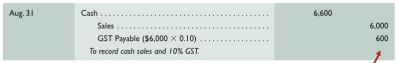
\includegraphics[width=1\columnwidth]{images/c10_sales_tax_payable.png}
		\caption{Harvey Norman is responsible for collecting 
			and paying the tax to the government. The company will debit Cash 
			for 
			\$6,600, the amount of the sale and the tax collected. Harvey 
			Norman 
			will credit Sales for \$6,000, and credit the current liability 
			account, GST Payable, for \$600. The GST tax is 10\% of the total 
			sale 
			of \$6,000. Harvey Norman will later debit the GST Payable Account 
			when 
			payment is made to the taxing authority.}	
	\end{figure}
	
	\subsubsection{Corporate Income Tax Payable}
	
	\textbf{Tax Payable} is calculated as the prevailing tax rates multiplied 
	by the profit before tax of the business. Corporate taxes may be paid in 
	instalments during the year. 
	
	\subsubsection{Unearned Revenues}
	
	Unearned revenues are amounts received in advance from customers for future 
	products or services e.g. Advance ticket sales for sporting events or music 
	concerts. An example is given below5: 
	
	\begin{figure}[ht]
		\centering
		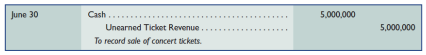
\includegraphics[width=1\columnwidth]{images/c10_unearned_revenues1.png}
		\caption{Assume that Beyonce sells \$5 million in tickets for eight 
			concerts. The entry debits Cash and credits Unearned Ticket Revenue}
		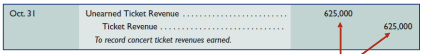
\includegraphics[width=1\columnwidth]{images/c10_unearned_revenues2.png}
		\caption{On October 31, Beyonce performs a concernt and Beyonce's 
			accountatn will debit, or reduce the Unearned Ticket Revenue, and 
			credit, or increase Ticket Revenue for \$625,000}
	\end{figure}
	
	\subsubsection{Notes Payable - Short-Term}
	
	Notes are a common form financing that are due within a year. They are 
	issued to borrow cash or purchase assets and may accrue interest expense 
	and interest payable at the end of the period. A \textbf{note payable} is a 
	written promise to pay a specific amount at a future date. A short-term 
	note payable pays the specific amount within one year or the company's 
	operating cycle, whichever is longer. Short-term notes bear interest. 
	
	\paragraph{Note Given to Extend Credit Period}. This is an example for 
	notes given to extend credit period:
	\begin{figure}[ht]
		\centering
		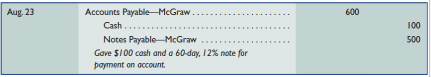
\includegraphics[width=1\columnwidth]{images/c10_notes_payable1.png}
		\caption{On August 23, Brady Company asks to extend its past-due \$600 
			account payable to McGraw. After some negotiations, McGraw agrees 
			to accept 
			\$100 Cash and a 60-day, 12\%, \$500 note payable to replace the 
			account. 
			Brady will debit or reduce, its Accounts Payable to McGraw and 
			decrease 
			Cahs for \$100 and credit, or increase, Notes Payable for \$500 to 
			McGraw}
		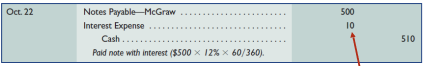
\includegraphics[width=1\columnwidth]{images/c10_notes_payable2.png}
		\caption{On October 22, Brady pays the note and all interest to McGraw. 
		To 
			prepare the journal entry on the books of Brady, we debit, or 
			decrease 
			Notes Payable to McGraw for \$500 and debit interest expense for 
			\$10. The 
			\$10 is interest at a 12\% annual rate for 60 days. Finally, the 
			Cash 
			account is credited, or decrease for the total of \$510.}
	\end{figure}	
	
	\paragraph{Note Given to Borrow from Bank}
	
	A bank nearly always require a borrower to sign a promissory note when 
	making a loan. When the loan matures, the borrower repays the note with an 
	amount larger than the amount borrowed. The difference between the amount 
	borrowed and the amount repaid is interest. This is a \textbf{promissory 
		note}:
	\begin{figure}[ht]
		%	\centering
		%	
		%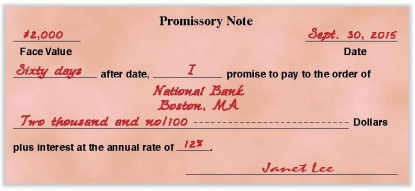
\includegraphics[width=0.6\columnwidth]{images/c10_promissory_note.png}
		%	\caption{There is a definite payee, National Bank in Boston and a 
		%	determinable of the payment, \$2000 plus interest at 12\% for 60 
		%days.}
		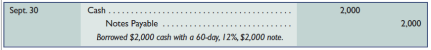
\includegraphics[width=1\columnwidth]{images/c10_promissory_note1.png}
		\caption{On Septemeber 30, a company needs \$2,000 and borrwos this 
		money 
			from the bank at 12\% annual interest. The loan is due in 60 days. 
			On the 
			date teh note was signed, the company debits Cash for \$,000 and 
			credit 
			Niotes Payable for the same amount.}
		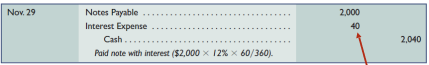
\includegraphics[width=1\columnwidth]{images/c10_promissory_note2.png}
		\caption{On November 29, the company repays the principle of the note 
		plus 
			interest. The company debits Note Payable and Interest Expense for 
			\$40. 
			Cash will be credited for \$2,040}
	\end{figure}
	
	If a short-term note payable is issued in one accounting period but it is 
	not payable until the following period. It is necessary to make an 
	adjusting entry at year-end to record the Interest Expense i.e. Figure 
	\ref{fig:eopap}:
	\begin{figure}[ht]
		\centering
		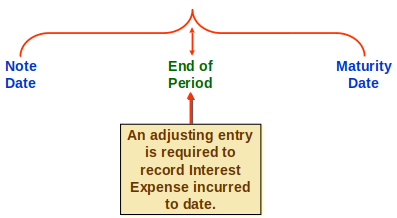
\includegraphics[width=0.8\columnwidth]{images/c10_end_period_note_adjustment.png}
		\caption{\label{fig:eopap}End-of-Period Adjustment to Notes}
		
		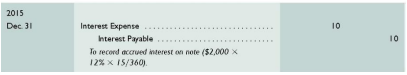
\includegraphics[width=1\columnwidth]{images/c10_end_note_adjustment1.png}
		\caption{On Dec 16, 2015, a company borrow \$2000 from a bnak at 12\% 
			interest for 60 days. An adjusting entry is needed on December 31 
			where 
			Interest Interest is debited by \$10 and Interest Payable is 
			credited 
			by \$10}
		
		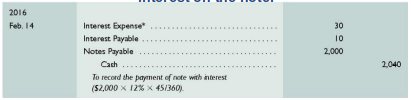
\includegraphics[width=1\columnwidth]{images/c10_end_note_adjustment2.png}
		\caption{On Feb 14, the Interest Expense is debited for \$30 i.e. 45 
			day interest and Interest Payable and Notes Payable is debited, and 
			Cash is credited for \$2,040.}
	\end{figure}
	
	\subsubsection{Payroll Liabilities}
	
	Employers incur expenses and liabilities from having employees. Employer 
	pay payroll tax expenses in connection with having employee on payroll. 
	These are not amounts withheld from the paycheck but are costs to the 
	employer. Fro example, in Singapore, under the law, both the employee and 
	employer have to contribute the Central Provident Fund (CPF), which is 
	primarily for the employee's retirement needs. From January 1, 2015, an 
	employee 50 years old and younger will have to contribute 20\%, which is 
	deducted from his salary and bonus, and paid into his account with the CPF 
	board.  His employer has to contribute 17\% to the employee's CPF account:
	
	\begin{figure}[ht!]
		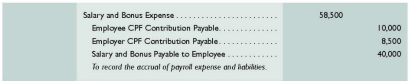
\includegraphics[width=1\columnwidth]{images/c10_employee_payroll.png}
		\caption{Assuming that the employee earns \$50,000 of salary and bonus 
			(the law states that only up to \$6,000 per month would attract CPF 
			contributions).}
	\end{figure}
	
	\subsection{Multi-Period Known Liabilities}
	
	When a known liability extends over multiple accounting periods, a portion 
	will be classified as current and a portion as a long-term liability. We 
	must make the adjusting entries at the end of each accounting period for 
	these multi-period liabilities. Two common multi-period liabilities include 
	subscriptions and long-term notes payable that have a portion maturing each 
	year. The current portion of long-term debt refers to that part of the 
	long-term debt due within one year or the operating cycle, whichever is 
	longer. 
	
	\begin{figure}[ht!]
		\centering
		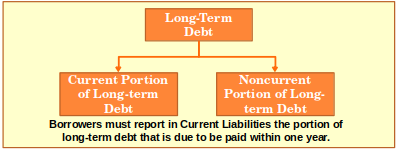
\includegraphics[width=0.9\columnwidth]{images/c10_long_term_liability.png}
	\end{figure}
	
	If a company borrows money with the promise to repay it within two years, 
	the loan is classified as a long-term debt. The company reports only the 
	accrued interest on the loan as a current liability in that year's balacne 
	sheet. After a yera has passed, the loan becomes a current liaiblity. When 
	this happens, the borrower must report teh loan in the Current Liabilities 
	section of the balance sheet. Rather than create a different account for 
	this, accountants simple remove the amount of princial to be repaid in the 
	upcoming year from the total long-term debt and report it as a current 
	liability, Current Portion of Long-term Debt.
	
	\subsection{Estimated Liabilities}
	
	Estimated Liabilitie are known obligations of an uncertain amount, but one 
	that cannot be reliaibly estimated. The amounts involved must be subjected 
	to reliable estimation before we may actually record an estimated 
	liability. 
	
	\textbf{Provisions} are liaiblities of uncertain timing and amount. It is 
	covered under IAS 37 - Provisions, Contingent Assets and Contingent 
	Liabilities. Companies may guarantee their products under a warranty that 
	may extend for 90 days to a year. The matching principle demands that the 
	company records the warranty expense in the same the buisness records safe 
	revenues. The exact amount of warranty expense cannot be known with 
	certainty. Hence, the business must estimate warranty expense and the 
	related liability.
	
	\subsubsection{Warranty Liabilities}
	
	Warranty liabiliteis are seller's obligations to replace or correct a 
	product (or service) that fails to perform as expected within a specified 
	period. to comply with full disclosure and matching principle, the seller 
	reports expected warranty expense in the period when revenue from the sale 
	is reported. An example for handling warranty liabilities is shown below:
	\begin{figure}[ht]
		\centering
		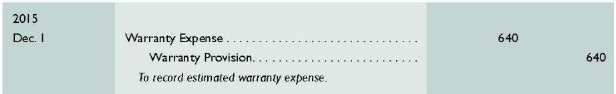
\includegraphics[width=1\columnwidth]{images/c10_warranty1.png}
		\caption{On Dec 1, 2015, a dealer sells a car for \$16,000 with a 
			maximum one-year or 12,000 mile warranty covering parts. Past 
			experience indicates warranty expenses average 4\% of car's selling 
			price}
		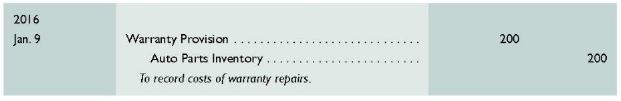
\includegraphics[width=1\columnwidth]{images/c10_warranty2.png}
		\caption{On Jan 9, 2016, the customer returns the car for repairs. The 
			dealer replaces parts costing \$200.}
	\end{figure}	
	
	\subsubsection{Contingent Liabilities}
	
	Contingent liabilities are potential liabiliteis that depend on future 
	outcome of past events i..e their ultimate resolution depends (is 
	contingent) on a future event:
	\begin{itemize}[noitemsep]
		\item Possible obligation to be confirmed by a future event
		\item Present obligation that may/may not require outflow of resources.
		\item Reliable estimate of amount of present obligation cannot be made. 
	\end{itemize}
	Contingent liabilites differ from other liabiltieis because tehri 
	dependence on a future event introduces a great deal of uncertainty. 
	Accounting for contingent liabilities depend on the likelihood that a 
	future event will occur and teh ability to estimate the future amount owed 
	if the event occurs. Accounting rules require the company to evaluate how 
	likely it is to have a real liability and if so, whetehr the amount of 
	liability can be reasonably estimated. 
	Future liabilities may arise due to lawsuits, tax disputes, or alleged 
	violation of environment protection laws. These liabilties can be accured, 
	disclosed or neither. The liability is handled using the following 
	guidelines: 
	\begin{figure}[ht]
		\centering
		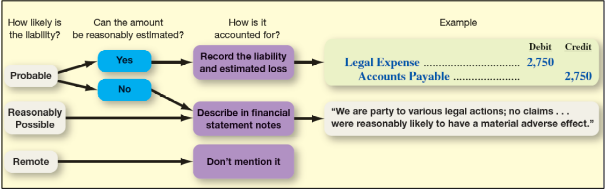
\includegraphics[width=1\columnwidth]{images/c10_contingent_liabilities.png}
		\caption{Contingent Liabilites}
	\end{figure}
	
	If the likelihood of occurence is determined to be possible, then the 
	contingency must be disclosed in the note sin the financial statements. 
	These are some common examples: 
	\begin{itemize}[noitemsep]
		\item \textbf{Potential Legal Claims} from Lawsuit - A potential claim 
		is recorded if the amount can be reliably estimated and payment for 
		damages are probable.
		\item \textbf{Debt Guarantees} - The guarantor usually discloses the 
		guarantee in its financial statement notes. If it is probable that the 
		debtor will default, the guarantor should record and report the 
		guarantee as a liability. If the original debtor fails to pay, the 
		obligation becomes the obligation of the guarantor. 
	\end{itemize}
	
	
	\subsection{Solvency}
	
	In evaluating a company's ability to pay its liabilities, a good place to 
	start is with the reports credit-rating agencies issue. We need to know how 
	to analyze a set of financial statements in the same way that a credit 
	rater would. Two financial ratios are commonly 
	used to assess a company's ability to generate resources to pay future 
	amounts owed:
	\begin{itemize}
		\item Debt-to-Assets Ratio - this ratio indicates the proportion of 
		total assets that are financed by liabilities. It is important to know 
		the proportion of assets financed by liabilities because liabilities 
		have to be repaid whether or not a company is doing well financially. 
		If assets are financed mainly by debt, rather than equity, then the 
		ratio will be high, which suggests that the company has adopted a risky 
		financing strategy e.g. a debt-to-assets ratio of 0.643 implies that 
		creditors have provided financing for nearly two-thirds of assets. 
		\begin{equation}
		\text{Debt-to-Assets Ratio} = \frac{\text{Total 
				Liabilities}}{\text{Total Assets}}
		\end{equation} 
		\item Times Interest Earned Ratio - this ratio tells us whether 
		sufficient resource are generated to cover interest costs. The higher 
		the ratio, the better the interest coverage e.g. a times interest 
		earned ratio of 9.19 means that \$9.19 of income (before the costs of 
		financing and taxes) is generated for each dollar of interest expense. 
		\begin{equation}
		\begin{aligned}
		&\text{Times Interest Earned Ratio} =\\ &\frac{\text{Net Income + 
				Interest Expense + Income Tax Expense}}{\text{Interest Expense}}
		\end{aligned}
		\end{equation}
	\end{itemize}
	
	\subsection{Statement of Cash Flows}
	
	The statement of cash flows helps users to determine how a company obtains 
	its cash and where it spends its cash. By providing this information, this 
	statement helps explain the change in cash balance from the beginning of 
	the period to the end of the period. 
	
	It is also important for users to know how a company funded its operations. 
	If so, users need to be aware of this so they can fully assess the cash 
	flow position of the company. Cash flow information is also useful to 
	determine if the business has sufficient cash to pay its debts or if the 
	business paid dividends during the period. 
	
	Cash includes currency and cash equivalents. \textbf{Cash equivalents} are 
	short-term, highly liquid investments that are easily converted into cash 
	and that have very little risk of loss e.g. short-term Treasury Bill that 
	is government-issued, is very close to maturity, and has very little risk 
	associated with it. 
	
	The Statement of Cash Flows includes the following three sections:
	\begin{itemize}[noitemsep]
		\item Operating Activities
		\item Investing Activities
		\item Financing Activities
	\end{itemize}
	
	\subsubsection{Operating Activities}
	
	The principal revenue-producing activities of the entity and other 
	activities that are not investing or financing activities. These generally 
	include those transactions and events that determine net profit. Examples 
	of inflows include:
	\begin{itemize}[noitemsep]
		\item Cash receipts from the sale of goods and the rendering of 
		services.
		\item Cash receipts from royalties, fees, commissions, and other 
		revenue.
	\end{itemize}
	Example of outflows include:
	\begin{itemize}[noitemsep]
		\item Cash payments to suppliers for goods 
		and services; 
		\item Cash payments to and on behalf of employees.
	\end{itemize}
	
	\subsubsection{Investing Activites}
	
	Investing activities involve the acquisition and disposal of long-term 
	assets and other investments not included in cash equivalents. Examples of 
	inflows include:
	\begin{itemize}[noitemsep]
		\item Sales of PPE, intangibles and other long-term assets
		\item Cash receipts from the sale of equity or debt instruments of 
		other entities.
		\item Cash receipts from the repayment of advances and loans made to 
		other parties.
	\end{itemize}
	Examples of outflows include: 
	\begin{itemize}[noitemsep]
		\item Cash payments to acquire PPE, intangibles and other long-term 
		assets.
		\item Cash payments to acquire equity or debt instruments of other 
		entities.
		\item Cash advances and loans made to other parties. 
	\end{itemize}
	
	\subsubsection{Financing Activities}
	
	Financing activities are those that result in changes in the size and 
	composition of the combined equity and borrowings of the entity. Examples 
	of inflows include:
	\begin{itemize}[noitemsep]
		\item Cash proceeds from issuing shares or other equity instruments.
		\item Cash proceeds from issuing debentures, loans, notes, bonds, 
		mortgages, and other short-term and long-term borrowings. 
	\end{itemize}
	Examples of outflows include:
	\begin{itemize}[noitemsep]
		\item Cash payments to owners to acquire or redeem the entity's shares.
		\item Cash repayments of the amounts borrowed. 
	\end{itemize}
	
	\subsubsection{Classification of Cash Flow Items}
	
	Reporting entities have choices in classifying interest and dividends. 
	Interest and dividends received may be classified as operating cash flows 
	because they enter into the determination of profit and loss. 
	Alternatively, interest and dividends received may be classified as 
	investing cash flows because they are returns on investments. Interest paid 
	may be operating or financing because it enters into the determination of 
	profits and is also a cost of obtaining financial resources. Dividends paid 
	may be classified as financing cash flow because they are a cost of 
	obtaining financial resource. Alternatively, dividends paid may be 
	classified as cash flows from operating activities in order to determine 
	the ability of an entity to pay dividends out of operating cash flows. 
	
	\begin{table}[ht]
		\centering
		\begin{tabular}{|p{0.30\columnwidth}||p{0.20\columnwidth}|
				p{0.20\columnwidth}|p{0.20\columnwidth}|}
			\hline 
			& Operating & Investing & Financing \\
			\hline 
			Interest received & Yes & Yes & \\
			\hline
			Dividends received & Yes & Yes & \\
			\hline
			Interest Paid & Yes & & Yes \\
			\hline
			Dividends Paid & Yes & & Yes \\
			\hline
		\end{tabular}
	\end{table}
	
	\subsubsection{Non-cash Investing and Financing}
	
	Some transactions involve investing activities and/or financing activities 
	with no cash. These items that require separate disclosure incude:
	\begin{itemize}[noitemsep]
		\item \textbf{Retirement of debt by issuing equity securities} e.g. 
		purchasing equipment and paying for it by issuing company shares. In 
		this transaction, the purchase of equipment is an investing activity 
		and the issuance of shares is a financing activity. Because no cash was 
		exchanged in this transaction ,it will not appear on the 
		statement of cash flows. Because of the significance and full 
		disclosure principle, these non-Cash investing and financing activities 
		must be disclosed in the financial statements or the note. 
		\begin{figure}[ht]
			\centering
			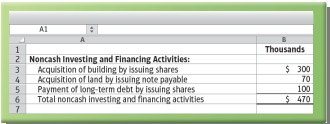
\includegraphics[width=0.9\columnwidth]{images/c10_noncash_investing_financing.png}
		\end{figure}
		\item \textbf{Conversion of preference shares into ordinary shares}. 
	\end{itemize}

	\subsection{Statement of Cash Flows Format}
	
	\begin{figure}[ht]
		\centering
		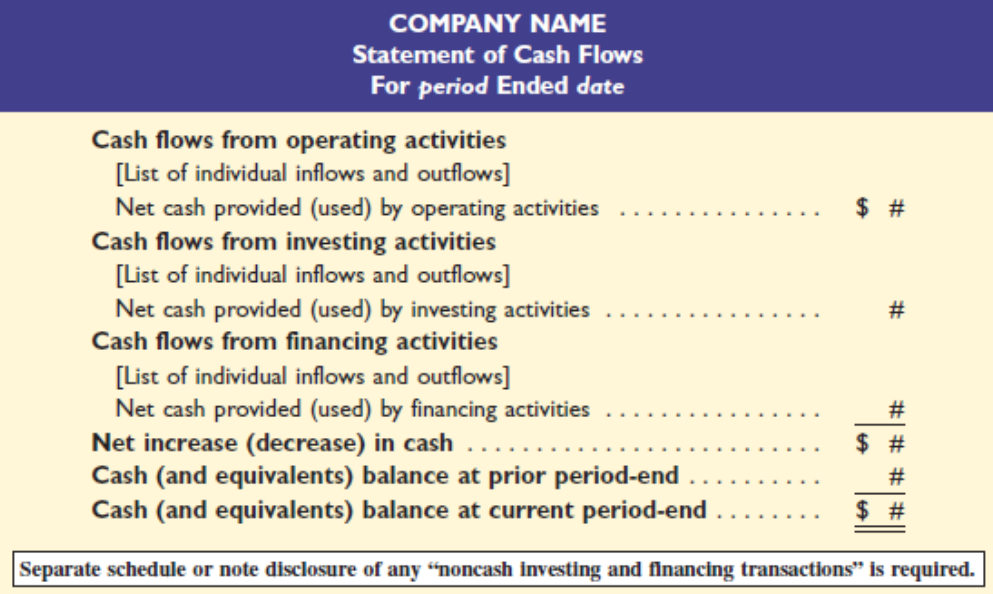
\includegraphics[width=\columnwidth]{images/c9/statement_of_cash_flows.png}
	\end{figure}
\end{document}